\documentclass[10pt,english,dvipsnames,aspectratio=169,handout]{beamer}\usepackage[]{graphicx}\usepackage[]{xcolor}
% maxwidth is the original width if it is less than linewidth
% otherwise use linewidth (to make sure the graphics do not exceed the margin)
\makeatletter
\def\maxwidth{ %
  \ifdim\Gin@nat@width>\linewidth
    \linewidth
  \else
    \Gin@nat@width
  \fi
}
\makeatother

\definecolor{fgcolor}{rgb}{0.345, 0.345, 0.345}
\newcommand{\hlnum}[1]{\textcolor[rgb]{0.686,0.059,0.569}{#1}}%
\newcommand{\hlstr}[1]{\textcolor[rgb]{0.192,0.494,0.8}{#1}}%
\newcommand{\hlcom}[1]{\textcolor[rgb]{0.678,0.584,0.686}{\textit{#1}}}%
\newcommand{\hlopt}[1]{\textcolor[rgb]{0,0,0}{#1}}%
\newcommand{\hlstd}[1]{\textcolor[rgb]{0.345,0.345,0.345}{#1}}%
\newcommand{\hlkwa}[1]{\textcolor[rgb]{0.161,0.373,0.58}{\textbf{#1}}}%
\newcommand{\hlkwb}[1]{\textcolor[rgb]{0.69,0.353,0.396}{#1}}%
\newcommand{\hlkwc}[1]{\textcolor[rgb]{0.333,0.667,0.333}{#1}}%
\newcommand{\hlkwd}[1]{\textcolor[rgb]{0.737,0.353,0.396}{\textbf{#1}}}%
\let\hlipl\hlkwb

\usepackage{framed}
\makeatletter
\newenvironment{kframe}{%
 \def\at@end@of@kframe{}%
 \ifinner\ifhmode%
  \def\at@end@of@kframe{\end{minipage}}%
  \begin{minipage}{\columnwidth}%
 \fi\fi%
 \def\FrameCommand##1{\hskip\@totalleftmargin \hskip-\fboxsep
 \colorbox{shadecolor}{##1}\hskip-\fboxsep
     % There is no \\@totalrightmargin, so:
     \hskip-\linewidth \hskip-\@totalleftmargin \hskip\columnwidth}%
 \MakeFramed {\advance\hsize-\width
   \@totalleftmargin\z@ \linewidth\hsize
   \@setminipage}}%
 {\par\unskip\endMakeFramed%
 \at@end@of@kframe}
\makeatother

\definecolor{shadecolor}{rgb}{.97, .97, .97}
\definecolor{messagecolor}{rgb}{0, 0, 0}
\definecolor{warningcolor}{rgb}{1, 0, 1}
\definecolor{errorcolor}{rgb}{1, 0, 0}
\newenvironment{knitrout}{}{} % an empty environment to be redefined in TeX

\usepackage{alltt}
\usepackage{fontspec}
\setsansfont[Mapping=tex-text]{Fira Sans}
\setcounter{secnumdepth}{4}
\setcounter{tocdepth}{4}
\usepackage[normalem]{ulem}
\usepackage[T1]{fontenc}
\usepackage{dcolumn}
\usepackage{booktabs}
\usepackage{bm}
\usepackage{setspace}
\makeatletter
\usetheme{metropolis}
\setbeamertemplate{frame footer}{Bosancianu | Schaub | Hertie School}
\setbeamerfont{page number in head/foot}{size=\tiny}
\setbeamercolor{footline}{fg=gray}
\usepackage{xcolor}
\setbeamercovered{dynamic}
\usepackage{tikz}
\usetikzlibrary{arrows, positioning,fit,shapes.misc}
\usepackage[labelformat=empty]{caption}
% For table captions in Beamer
\usepackage[sectionbib]{apacite}
\renewcommand{\bibliographytypesize}{\footnotesize}
\makeatletter
\let\st@rtbibsection\@bibnewpage
\let\st@rtbibchapter\@bibnewpage
\makeatother
\usepackage{amsmath, mathtools}
\usepackage{xunicode}
\usepackage{hyperref}
\usepackage{pgfplots}
\makeatletter
\long\def\ifnodedefined#1#2#3{%
    \@ifundefined{pgf@sh@ns@#1}{#3}{#2}%
}
\pgfplotsset{
    discontinuous/.style={
    scatter,
    scatter/@pre marker code/.code={
        \ifnodedefined{marker}{
            \pgfpointdiff{\pgfpointanchor{marker}{center}}%
             {\pgfpoint{0}{0}}%
             \ifdim\pgf@y>0pt
                \tikzset{options/.style={mark=*}}
                \draw [densely dashed] (marker-|0,0) -- (0,0);
                \draw plot [mark=*,mark options={fill=white}] coordinates {(marker-|0,0)};
             \else
                \ifdim\pgf@y<0pt
                    \tikzset{options/.style={mark=*,fill=white}}
                    \draw [densely dashed] (marker-|0,0) -- (0,0);
                    \draw plot [mark=*] coordinates {(marker-|0,0)};
                \else
                    \tikzset{options/.style={mark=none}}
                \fi
             \fi
        }{
            \tikzset{options/.style={mark=none}}        
        }
        \coordinate (marker) at (0,0);
        \begin{scope}[options]
    },
    scatter/@post marker code/.code={\end{scope}}
    }
}
\makeatother
% Defines a checkmark
\def\checkmark{\tikz\fill[scale=0.4,color=orange](0,.35) -- (.25,0) -- (1,.7) -- (.25,.15) -- cycle;}
\newcommand{\indep}{\perp \!\!\!\! \perp}
\setbeamertemplate{itemize items}{\checkmark}
\usepackage{multirow}
\hypersetup{pdfauthor={Bosancianu and Schaub},
	pdftitle={Statistical Modeling and Causal Inference with R},
	pdfsubject={Week 9: Panel Data},
	pdfkeywords={Berlin, Hertie, 2020, week 9, RDD}}
\title{\textsc{Statistical Modeling and Causal Inference with R}}
\subtitle{Week 9: Panel Data}
\date{November 9, 2020}
\author{Manuel Bosancianu \hfill Max Schaub}
\institute{Hertie School of Governance}
\IfFileExists{upquote.sty}{\usepackage{upquote}}{}
\begin{document}
\maketitle





\section{Applied example}

\begin{frame}
  \frametitle{SOEP structure}
  Example taken from \citeA{bruderl_fixed_2015}, based on SOEP.\bigskip

  Standard setup for panel data:
  
  \begin{itemize}
    \item sample of households, with everyone in HH interviewed (including foreigners)
    \item ongoing since 1984 (expanded in 1990 to cover former GDR)
    \item annual interviews (occasionally, top-up households added)
    \item expanded again in 2016 to cover refugees
  \end{itemize}
  
\end{frame}


\begin{frame}
  \frametitle{Extensive potential}
  \begin{itemize}
    \item social inequalities
      \begin{enumerate}
        \item perceptions on incomes
        \item social mobility
        \item changes in income distribution
      \end{enumerate}
  \end{itemize}
  
  \pause
  
  \begin{itemize}
    \item well-being and health
      \begin{enumerate}
        \item impact of Covid-19
        \item impact of aging
      \end{enumerate}
  \end{itemize}
  
  \pause
  
  \begin{itemize}
    \item migrant integration
      \begin{enumerate}
        \item language skills and job market success
        \item requalification in host country
        \item success of second generation
      \end{enumerate}
  \end{itemize}  
  
\end{frame}


\begin{frame}
  \frametitle{Impact of marriage}
  Impact of first marriage on life satisfaction?\bigskip
  
  Problem: happier people are more likely to get married \cite{frey_happiness_2005}.\bigskip
  \pause
  
  Similarities re. self-selection: impact of institutions on development.\bigskip
  \pause
  
  Variables:
  
  \begin{columns}
  \scriptsize
  	\begin{column}{0.48\textwidth}
		\begin{itemize}
		  \item \textcolor{orange}{id}: person ID
		  \item \textcolor{orange}{year}: wave
		  \item \textcolor{orange}{marry}: married
		  \item \textcolor{orange}{yrsmarried}: marriage length
		\end{itemize}
	  \end{column}
	\begin{column}{0.48\textwidth}
	  \begin{itemize}
	    \item \textcolor{orange}{age}: R.'s age
		  \item \textcolor{orange}{loghhinc}: HH income (log)
		  \item \textcolor{orange}{woman}: gender 
		  \item \textcolor{orange}{happy}: life satisfaction
	  \end{itemize}
	\end{column}
\end{columns}
  
\end{frame}


\begin{frame}
  \frametitle{Who to include?}
  Any unit who can potentially change from not-treated to treated \cite{bruderl_fixed_2015, sobel_does_2012}.\bigskip
  \pause
  
  If unit's treatment status changed during period, they get included.
  
  If unit never got treatment, they get included (control group).\bigskip
  \pause
  
  What about already treated? If treatment effect varies over time, including them might bias estimation (older vs. younger).
\end{frame}


\begin{frame}
  \frametitle{Data format}




  
  \begin{figure}
  \caption{Trajectory of 8 units}
  \begin{center}
      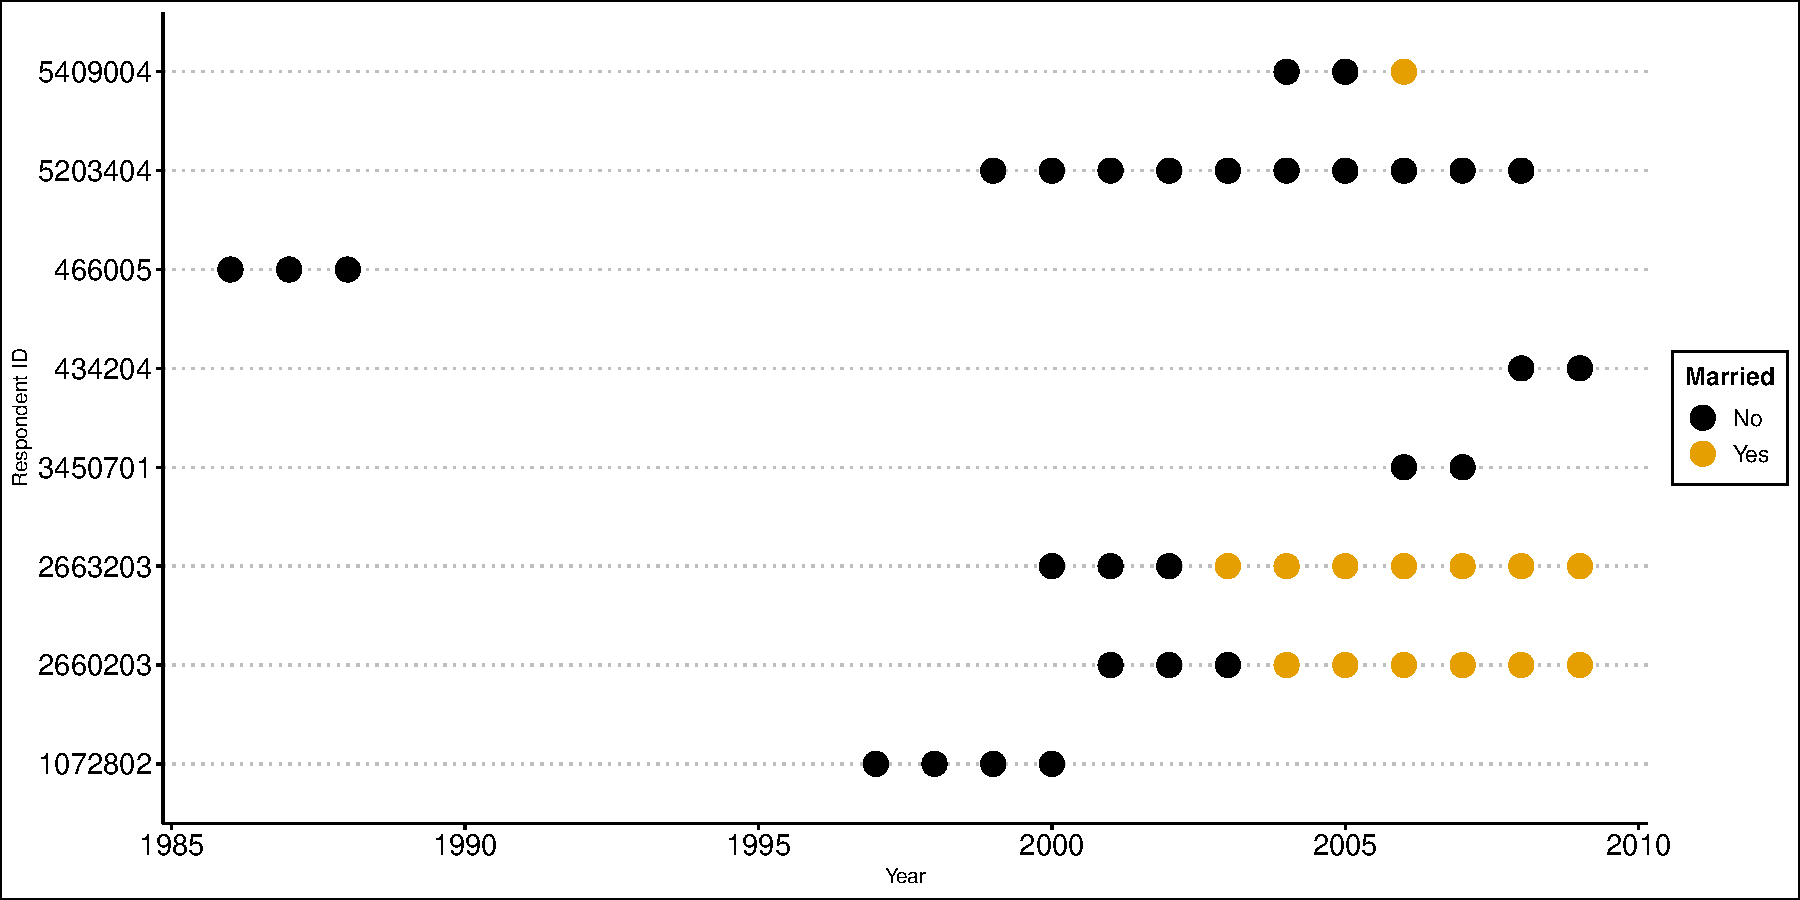
\includegraphics[scale=0.35]{../04-figures/09/05.pdf}
  \end{center}
  \label{fig:01}
  \end{figure}
  
\end{frame}


\begin{frame}
  \frametitle{Explore variation}
  How is the ratio ``between-unit / within-unit'' in terms of variation?\bigskip
  
\begin{table}[!ht]
\centering
\begin{tabular}{c c c c}
\toprule
    & Gender & Satisfaction & Marriage \\
\midrule
Mean               & 0.467 & 7.147 & 0.230  \\
$\sigma_{within}$  & 0     & 1.260 & 0.267  \\
$\sigma_{between}$ & 0.499 & 1.282 & 0.269  \\  
\bottomrule
\end{tabular}
\label{tab:01}
\end{table}

  Gender doesn't have any within-unit variation for us.
  
\end{frame}


\section{Fixed effects specifications}

\begin{frame}
  \frametitle{Unit FEs}
  We can't use gender in this specification.



 
 \begin{table}
\begin{center}
\begin{tabular}{l D{.}{.}{6.6}}
\toprule
 & \multicolumn{1}{c}{DV: satisfaction} \\
\midrule
Marriage        & 0.167^{***}  \\
                & (0.017)      \\
HH income (log) & 0.125^{***}  \\
                & (0.009)      \\
Age             & -0.041^{***} \\
                & (0.001)      \\
\midrule
R$^2$           & 0.016        \\
Adj. R$^2$      & -0.119       \\
Num. obs.       & 121919       \\
\bottomrule
\multicolumn{2}{l}{\scriptsize{$^{***}p<0.001$; $^{**}p<0.01$; $^{*}p<0.05$}}
\end{tabular}
\label{tab:02}
\end{center}
\end{table}
  
\end{frame}


\begin{frame}
  \frametitle{Unit and period FEs}
  Can't add either gender or age in this model.





\begin{table}
\begin{center}
\begin{tabular}{l D{.}{.}{6.6}}
\toprule
 & \multicolumn{1}{c}{DV: satisfaction} \\
\midrule
Marriage        & 0.163^{***} \\
                & (0.017)     \\
HH income (log) & 0.126^{***} \\
                & (0.009)     \\
\midrule
R$^2$           & 0.003       \\
Adj. R$^2$      & -0.134      \\
Num. obs.       & 121919      \\
\bottomrule
\multicolumn{2}{l}{\scriptsize{$^{***}p<0.001$; $^{**}p<0.01$; $^{*}p<0.05$}}
\end{tabular}
\label{tab:03}
\end{center}
\end{table}

\end{frame}


\begin{frame}[fragile]
  \frametitle{Should we trust SE?}
  Assumption for errors is $\upsilon_{it} \sim iid(0, \sigma_{\upsilon}^2)$.\bigskip
  
  With longer panels, serial correlation between errors is a problem: $Cor(\upsilon_{it}, \upsilon_{i(t-1)}) \neq 0$.\bigskip
  \pause
  
\begin{knitrout}\scriptsize
\definecolor{shadecolor}{rgb}{0.969, 0.969, 0.969}\color{fgcolor}\begin{kframe}
\begin{alltt}
\hlkwd{pbgtest}\hlstd{(model2,} \hlkwc{order} \hlstd{=} \hlnum{2}\hlstd{)}
\end{alltt}
\begin{verbatim}

	Breusch-Godfrey/Wooldridge test for serial correlation in panel models

data:  happy ~ marry + loghhinc
chisq = 473.01, df = 2, p-value < 2.2e-16
alternative hypothesis: serial correlation in idiosyncratic errors
\end{verbatim}
\end{kframe}
\end{knitrout}
  
  Manual correction needed.
\end{frame}



\begin{frame}[fragile]
  \frametitle{Robust standard errors}
  Correction done on SEs to factor in serial correlation.
  
\begin{knitrout}\scriptsize
\definecolor{shadecolor}{rgb}{0.969, 0.969, 0.969}\color{fgcolor}\begin{kframe}
\begin{alltt}
\hlkwd{coeftest}\hlstd{(model2,}
         \hlkwc{vcov.} \hlstd{=} \hlkwa{function}\hlstd{(}\hlkwc{x}\hlstd{)} \hlkwd{vcovHC}\hlstd{(x,} \hlkwc{type} \hlstd{=} \hlstr{"sss"}\hlstd{))}
\end{alltt}
\begin{verbatim}

t test of coefficients:

         Estimate Std. Error t value  Pr(>|t|)    
marry    0.163145   0.022726  7.1789 7.072e-13 ***
loghhinc 0.125558   0.012250 10.2497 < 2.2e-16 ***
---
Signif. codes:  0 '***' 0.001 '**' 0.01 '*' 0.05 '.' 0.1 ' ' 1
\end{verbatim}
\end{kframe}
\end{knitrout}
  
\end{frame}


\section{Random effects specification}

\begin{frame}
  \frametitle{Random effects logic}

\begin{equation}
\footnotesize
  \begin{cases}
  Happy_{it} = \beta_{i0} + \beta_{1}*Marriage_{it} + \beta_{2}*Age_{it} + \beta_{3}*Income_{it} + \epsilon_{it} \\
  \beta_{i0} = \gamma_{00} + \gamma_{01}*Gender_{i} + \upsilon_{i}
  \end{cases}
\end{equation}
  \pause

  The unit fixed effects (actually, the intercepts) are modeled with 2nd equation.\bigskip
  \pause
  
  Goal is to explain their variance (instead of treating them as nuisance).
  
\end{frame}


\begin{frame}
  \frametitle{REs results}
  
\begin{knitrout}\scriptsize
\definecolor{shadecolor}{rgb}{0.969, 0.969, 0.969}\color{fgcolor}\begin{kframe}
\begin{alltt}
\hlstd{model3} \hlkwb{<-} \hlkwd{plm}\hlstd{(happy} \hlopt{~} \hlstd{marry} \hlopt{+} \hlstd{loghhinc} \hlopt{+} \hlstd{age} \hlopt{+} \hlstd{woman,}
              \hlkwc{index} \hlstd{=} \hlkwd{c}\hlstd{(}\hlstr{"id"}\hlstd{,}\hlstr{"year"}\hlstd{),}
              \hlkwc{effect} \hlstd{=} \hlstr{"twoways"}\hlstd{,}
              \hlkwc{model} \hlstd{=} \hlstr{"random"}\hlstd{,}
              \hlkwc{data} \hlstd{= df.happy)}
\end{alltt}
\end{kframe}
\end{knitrout}
  
 Function specifies random effects, as well as shape of correlation.\bigskip
 \pause
 
 Serial correlation of errors still needs to be addressed.
  
\end{frame}


\begin{frame}
  \frametitle{REs results}
  

  
 \begin{table}
\begin{center}
\footnotesize
\begin{tabular}{l D{.}{.}{6.6}}
\toprule
 & \multicolumn{1}{c}{DV: satisfaction} \\
\midrule
(Intercept)     & 5.736^{***}  \\
                & (0.069)      \\
Marriage        & 0.134^{***}  \\
                & (0.011)      \\
HH income (log) & 0.193^{***}  \\
                & (0.006)      \\
Age             & -0.020^{***} \\
                & (0.001)      \\
Woman           & 0.058^{***}  \\
                & (0.015)      \\
\midrule
s\_idios        & 1.331        \\
s\_id           & 1.048        \\
s\_time         & 0.087        \\
R$^2$           & 0.023        \\
Adj. R$^2$      & 0.023        \\
Num. obs.       & 121919       \\
\bottomrule
\multicolumn{2}{l}{\scriptsize{$^{***}p<0.001$; $^{**}p<0.01$; $^{*}p<0.05$}}
\end{tabular}
\label{tab:04}
\end{center}
\end{table}
  
\end{frame}



\section{Other questions}

\begin{frame}
  \frametitle{Same design, different question}
  
  What is the impact of social media use on mental health, e.g. depression?
  
\begin{figure}
\begin{center}
    
\includegraphics[scale=0.5]{../04-figures/09/06.PNG}
\end{center}
\label{fig:02}
\end{figure}
  
\end{frame}


\begin{frame}
  \frametitle{No clear-cut answer yet}
  
  \begin{figure}
\begin{center}
    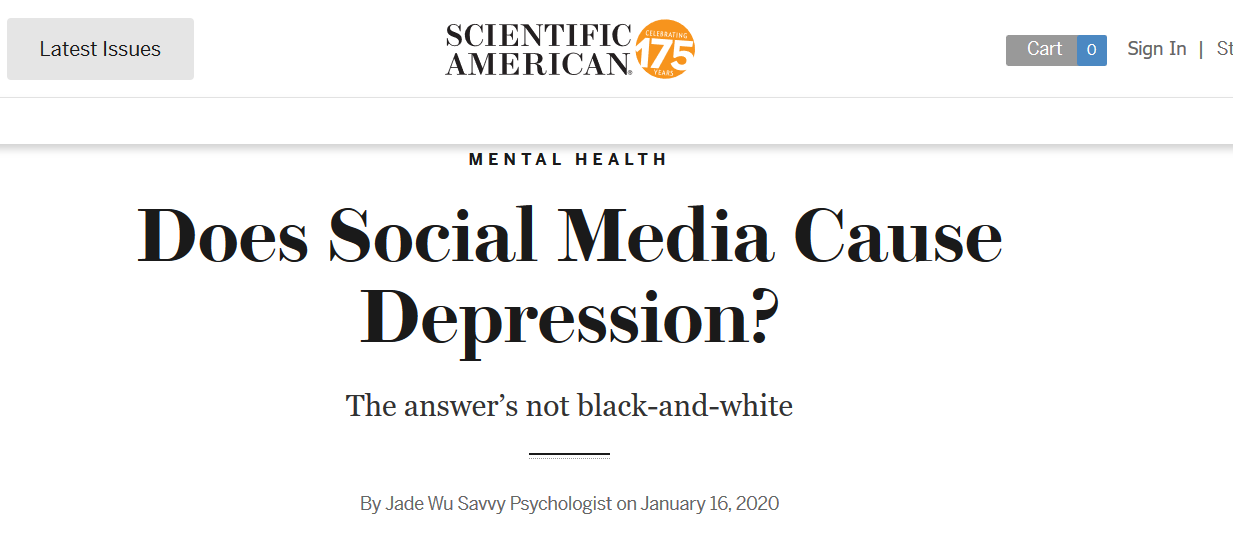
\includegraphics[scale=0.4]{../04-figures/09/07.PNG}
\end{center}
\label{fig:03}
\end{figure}
  
\end{frame}


\begin{frame}
  \frametitle{Discussion topics}
  
  \begin{itemize}
  \setlength\itemsep{1.5em}
    \item How would you design a study to assess this?
    \item What variables would you need to study this?
    \item How often do you need to collect data for this design?
    \item What is treatment and comparison group?
  \end{itemize}
  
\end{frame}

% END
\begin{frame}
\begin{center}
    \Huge Thank \textcolor{orange}{you} for the kind attention!
\end{center}
\end{frame}

% REFERENCES %

\begin{frame}[allowframebreaks, plain]
\bibliographystyle{apacite}
\scriptsize\bibliography{../Bibliography}
\end{frame}

\end{document}
